\section{相关工作}
\label{sec:works}

\subsection{双倍行距的审阅模式}
% 先讲一下为什么 edit 模式是双倍行间距，这个就不得不讲我用 AEA 的模版写 paper 的时候了，套上模版感觉哪里不对劲，然后发现它有一个审阅的模式，这东西是真好，真的好，真的真的真的好。
本项目建议在写作时采用审阅模式（\texttt{edit}），这一设计源于我在使用美国经济学会（American Economic Association，AEA）的 \LaTeX{} 模板写作时的体验。
AEA 为投稿作者提供了审阅模式，并要求使用其模板准备投稿稿件时采用该模式。\footnote{AEA 模板说明见 \url{https://www.aeaweb.org/journals/templates}。}
初次套用模板时，我注意到稿件的行距明显变大，后来才发现这是审阅模式的排版设置。
较宽的行距让阅读和批注有了更多空间，也方便作者逐段检查和修改。
因此，本项目在审阅模式中采用双倍行距，作为研究者撰写、讨论和修改稿件时的默认版式。

对我个人而言，我喜欢将论文打印出来，用纸笔阅读和修改。
纸质稿上的批注可以直接写在需要调整的句子旁边，遇到需要重新组织的论证，也可以在段落间标记调整思路。
双倍行距为这些修改留出了书写空间，使添加词句、修改措辞和标记问题时不必将文字挤在一起。
对于需要多轮修改的稿件，这样的排版也方便作者回看此前留下的批注。

在对研究者的调研中，我发现，喜欢打印稿件阅读和修改的并不只有我一人。
他们同样需要在纸质稿上留出批注和修改的空间。
这意味着，审阅版式需要考虑纸笔修改的空间。
双倍行距的审阅模式为这些研究者提供了一份适合打印批注的稿件，也让纸质审阅中留下的意见更容易在后续修订时辨认和整理。

现有文献也能支持打印的纸质版是文献阅读的一种主要方式。
\textcite{tenopir_international_2019} 在 2018 年开展了一项国际调查，要求受访者回忆最近一次阅读学术文章的方式。
在回答该问题的 366 名受访者中，有 133 人将下载的文章打印后阅读，占比约 36.3\%。
调查共获得 606 份有效回应，其中约三分之一的受访者来自社会科学领域，但作者指出该样本可能不具代表性。
在另一项芬兰调查中，\textcite{tenopir_finland_2019} 记录了研究者于 2016 年报告的最近一次期刊文章阅读经历。
在 455 次阅读中，40.4\% 是将下载的文章打印后阅读，另有 5.3\% 直接阅读纸质期刊。
这些结果表明，纸质阅读在两项调查记录的学术阅读中占有一定比例，为关注研究者的纸质阅读需求提供了经验依据。

纸质批注也出现在已有调查中。
\textcite{lincoln_reading_2013} 对神学和宗教研究领域的图书馆用户进行调查，发现教授或讲师受访者中有 53\% 表示经常在纸质文章上批注或标记重点。
在德国职业教育与培训研究领域的调查中，\textcite{getz_researchers_2021} 报告有 63.6\% 的受访者同意或倾向同意，自己阅读纸质材料时比阅读屏幕上的数字出版物更专注。
对于习惯纸质阅读和批注的研究者，审阅模式可以直接生成双倍行距稿件，使得打印后的阅读效果更舒服。

\subsection{Agent Skill}

Agent Skill 是由 Anthropic 于 2025 年推出的一种面向 AI Agent 提供特定任务知识与操作流程的开放格式。
一个 Skill 通常以文件夹的形式组织，其中的 \texttt{SKILL.md} 文件描述该技能的名称、用途和执行说明，也可以附带脚本、参考资料或模板等资源。\footnote{更多信息详见 \url{https://agentskills.io} 和 \url{https://github.com/anthropics/skills}。}
当用户的任务与某项技能相关时，Agent 可以读取相应说明和所需资源，并据此完成任务。
这种组织方式使研究者能够将常用的操作步骤和领域知识保存下来，在后续任务中重复使用。


在实际写作中，\LaTeX{} 的编译命令和环境配置并不容易记住，遇到又臭又长的报错日志时，找到问题所在也可能需要花费不少时间。
有一天我发现，ChatGPT Desktop 中有一个 OpenAI 发布的 LaTeX 插件，可以协助处理这些工作（见图~\ref{fig:latex-plugin-openai}）。\footnote{如果你的 ChatGPT 里还没有这个插件，可以尝试发送这样的提示词：“请从 \url{https://chatgpt.com/plugins/share/latex@openai-bundled} 安装 LaTeX 插件，并帮我检查我的 LaTeX 环境是否准备就绪。”}
这个插件包含三个 Skill：\texttt{latex-doctor} 用于检查编译环境和工具是否可用，\texttt{latex-compile} 用于编译稿件，\texttt{texlive-runtime-installer} 则在没有检测到可用的 TeX Live 或 MacTeX 时，帮助安装完整的 TeX Live 环境。
借助这些技能，研究者可以用自然语言请 Agent 检查环境、编译文件并协助分析报错，把更多精力放在论文内容上。

\begin{figure}[htbp]
    \centering
    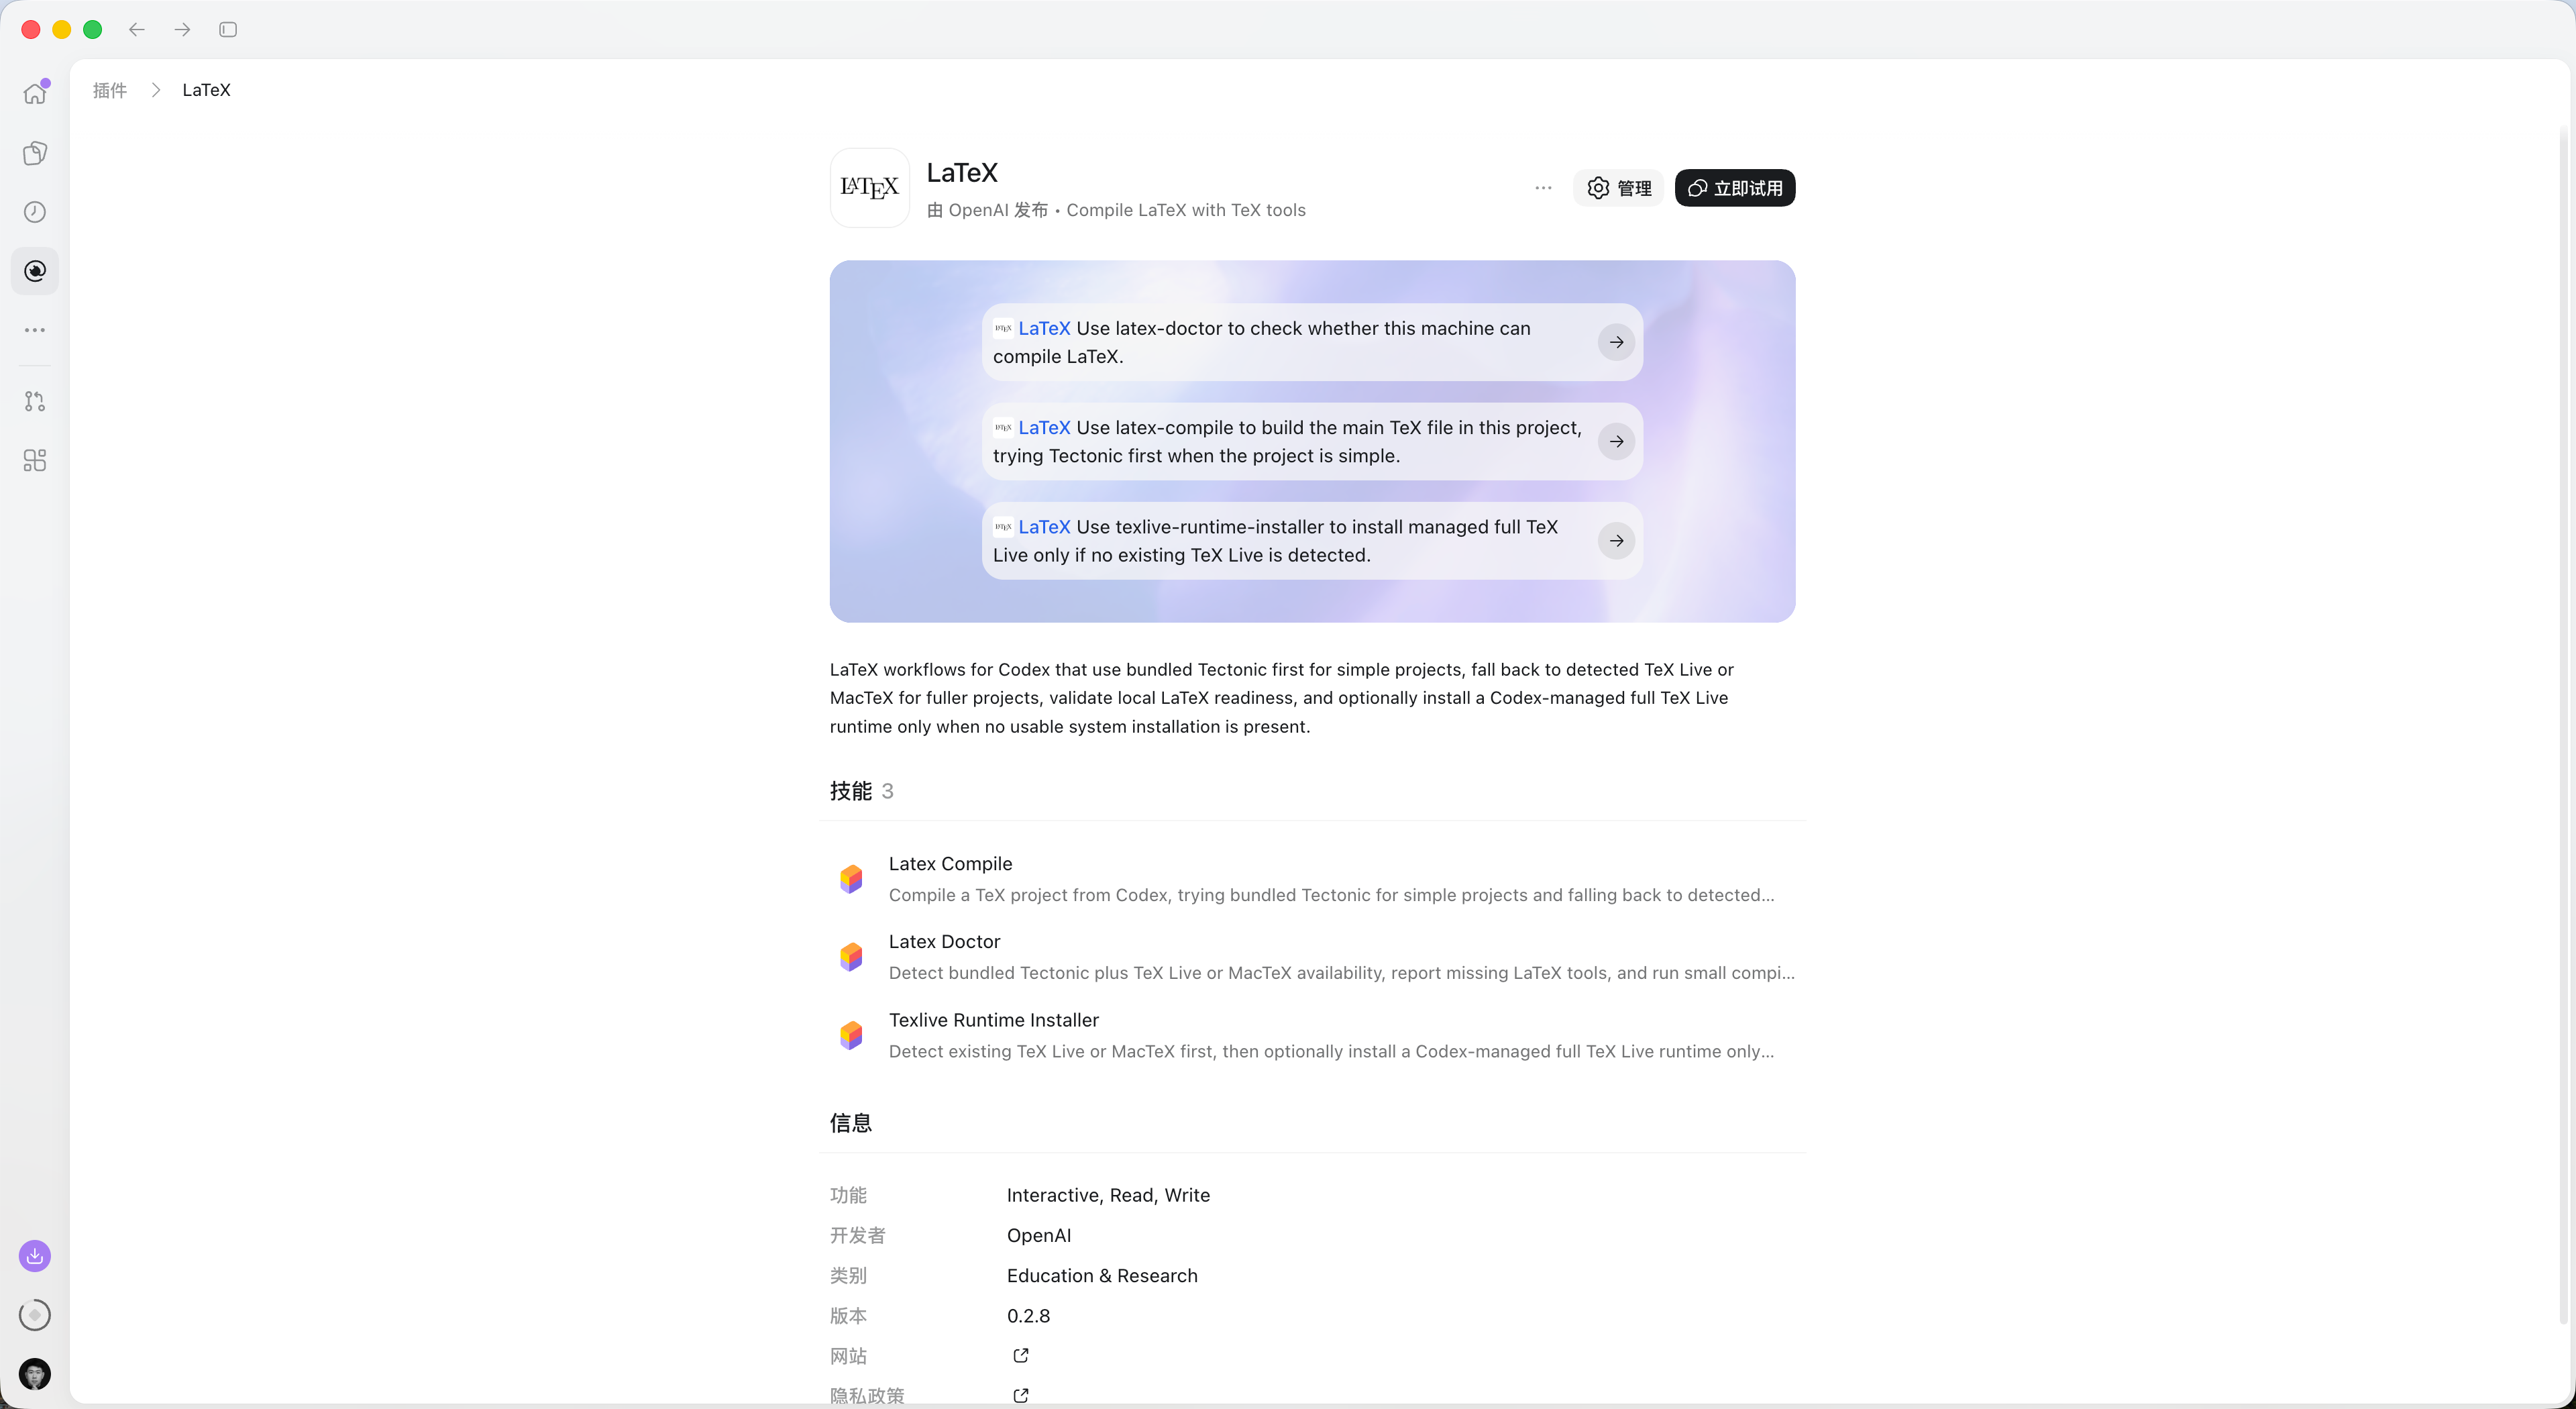
\includegraphics[width=\linewidth]{figs/latex-plugin-openai.png}
    \caption{OpenAI 发布的 \LaTeX{} 插件及其附带的三个 Skill}
    \label{fig:latex-plugin-openai}
\end{figure}


同时，因为我并没有找到特别好用特别适合我的 Skill 来帮我处理具体的命令。
因为我记不住 \LaTeX{} 的命令，所以我需要借助于 AI 帮我写很多的命令。但当我处于无网络的情况下我不得不依赖于我在本地部署的模型，可他们的能力却一言难尽。
因此，在我开源的一套 Agent Skill 里有一个专门的 Skill 就是针对于如何编写 \LaTeX{} 代码。
该 Skill 面向论文写作中常见的 \LaTeX{} 代码编写任务，整理了公式、图表和文献引用等场景的基本写法及注意事项。\footnote{项目地址为 \url{https://github.com/sepinetam/sepine-research-skill}。如需安装只需要将下面这段话发给你的 Agent：“帮我安装 Sepine 的 Research Skill，地址在 https://github.com/sepinetam/sepine-research-skill”}
使用时，我们只需要用自然语言讲出我们需要什么样的效果，Agent 即可结合 Skill 中的说明生成或修改相应代码。
对于本地部署的模型，这些说明也可以作为完成任务时的参考，帮助它按照项目约定处理常见的 \LaTeX{} 命令。

\subsection{Coding Agent}

Coding Agent 是一种能够围绕用户提出的任务，结合项目文件编写、修改和运行代码的 AI Agent。
研究者可以用自然语言描述问题，让它读取相关文件、生成程序、执行命令，并根据运行结果继续调整。
在论文写作场景中，这种工作方式也可以用于编辑 \LaTeX{} 源码、编译稿件和排查编译错误。

\textcite{lyttelton_coding_agents_2026} 对 1,260 名定量社会科学研究者开展的基线调查发现，81\% 的受访者曾在研究中使用生成式 AI，而约 20\% 经常使用 Coding Agent。
研究同时指出，受访者是为一项提供 Claude 使用机会的研究招募的，并不构成具有代表性的总体样本。
另一项研究中，\textcite{hermle_scientific_discovery_2026} 分析了 207,000 个 Claude 和 Claude Code 科研会话，发现数据分析约占 Claude Code 科研会话的一半。
这些结果反映了研究者使用相关工具的场景，为理解 Coding Agent 在科研工作中的应用提供了线索。

在研究的具体环节中，AI Agent 可以围绕数据、代码和运行结果协助研究者完成任务。
例如，在数据整理阶段，\textcite{li_autodcworkflow_2025} 构建了 AutoDCWorkflow，根据原始表格和分析目的生成数据清洗步骤，并在涵盖 96 张表格、142 个分析目的的测试集中评估了结果。
在研究复现阶段，\textcite{shah_reproducibility_2026} 以五项原本可以复现的社会科学研究为基础，人为加入缺失软件包、文件路径错误等问题，考察 Agent 检查文件、修改代码并重新运行分析的能力。
在这组受控测试中，Agent 方案在不同难度下的复现成功率为 69\%--96\%，展示了它协助处理分析流程中具体错误的可能性。
从数据整理到程序运行和复现检查，这些工作为研究者如何借助 Agent 处理实证研究中的重复性任务提供了参考。
研究者仍需要结合研究问题判断数据处理规则、样本与模型设定，并检查 Agent 生成的代码和结果。

对于希望在研究中使用 Coding Agent 的研究者，目前已经有几种通用工具可以选择。
目前比较主流的解决方案详见表~\ref{tab:agents}，其中主要推荐的智能体有 ChatGPT Desktop 和 DeepSeek Harness。\footnote{这两个 Agent Harness 的推荐考量是从可用性和可付费性两个角度。我们不得不承认 Claude 很强，但受限于某些许可的原因身处于中国大陆的用户不能够进行购买和使用，但与之相对应的 ChatGPT 就会缓和很多，可以相对轻松地使用上和订阅上。DeepSeek Harness 是完全开源的 Harness 框架，其推荐原因是它的新颖性和被爱包裹，一个在爱中长大的孩子，被整个社区用爱投喂，它差不到哪去。}
ChatGPT Desktop 中有两种模式，分别为 ChatGPT 和 Codex，我们可以简单地用一个通俗的方式去理解，ChatGPT 主要赋能工作场景（或轻代码场景），聚焦于将重复化的工作流自动化；Codex 更多赋能于编码场景。对于研究者来说，如果是资深研究者可以考虑从 ChatGPT 模式切入，在协作工作中把固定的流程自动化。
DeepSeek Harness 我们可以简单地理解成电脑界的 Linux，手机界的 Android，（汽车界的 Tesla？）它有高度化的自定义能力，适合喜欢折腾的研究者。它就好像是给你一间毛坯房，你可以自由地配置任何事物只要你能想到。

\begin{table}[htbp]
    \centering
    \caption{几种 AI Agent 工具的比较}
    \label{tab:agents}
    \zihao{5}
    \setlength{\tabcolsep}{3pt}
    \begin{tabular}{@{}p{0.19\linewidth}p{0.16\linewidth}p{0.39\linewidth}p{0.20\linewidth}@{}}
        \toprule
        \textbf{名称} & \textbf{来源} & \textbf{特点} & \textbf{可获得性} \\
        \midrule
        ChatGPT & OpenAI & Codex 内核开源 & \ding{72}\ding{72}\ding{72}{\color{gray}\ding{72}\ding{72}} \\
        \addlinespace[2pt]
        Claude & Anthropic & Claude Code 编程与命令执行 & \ding{72}{\color{gray}\ding{72}\ding{72}\ding{72}\ding{72}} \\
        \addlinespace[2pt]
        DSH & DeepSeek & 完全开源、一切皆插件 & \ding{72}\ding{72}\ding{72}\ding{72}\ding{72} \\
        \addlinespace[2pt]
        WorkBuddy & 腾讯 & 办公与文件处理 & \ding{72}\ding{72}\ding{72}\ding{72}\ding{72} \\
        \addlinespace[2pt]
        豆包工作 & 字节跳动 & 办公与飞书生态 & \ding{72}\ding{72}\ding{72}\ding{72}\ding{72} \\
        \addlinespace[2pt]
        Marx Max & AIdea-Labs & 专为社科研究者制作 & \ding{72}\ding{72}\ding{72}\ding{72}{\color{gray}\ding{72}} \\
        \bottomrule
    \end{tabular}
    \par\smallskip
    {\footnotesize\raggedright
    \textbf{注：}可获得性满分五颗星，黑色星表示所得星数，灰色星表示其余星数。\par}
\end{table}


除此之外，我们在打造一个专门为社会科学研究者服务的 AI 原生科研工作台。\footnote{目前仍在开发测试阶段，欢迎有兴趣的研究者来尝试使用，产品名字暂定为 Marx Max，名字的灵感源自两位社会科学的巨人，卡尔·马克思和马克思·韦伯。详见\href{https://marx-max.aidea-labs.com/?source_utm=econ-sbm-template}{\underline{\textit{产品官网}}}}
在该产品中，我们将对话、文件系统、科学计算、文献管理等科研常用工具集成在同一个桌面环境，它可以视为社会科学版的 Claude Science，让研究者能够围绕自己的数据、代码和稿件等内容在同一处推进。
该项目的出发点是不希望让“贩卖焦虑”的自媒体对科研产生不当的影响。
我自己平时刷手机的时候，发现很多的账号在渲染一种“再不学习就被淘汰了”的观点，起初我以为不会有人陷入其中，但是事实却让我愕然。
我认为，当下的 AI 对于研究者来说是一种“现在不学就不需要学”的状态，因为技术的变化实在是太快了，我们不可能在研究之外每天都去追最新的技术，而如果晚一两周再去看一项新技术的话，它可能已经被革新了。

故此，我希望能够让技术平权，让每一个研究者可以专注于自己的研究上而非被这种 FOMO 的情绪左右。
我们不希望让它们渲染这种情绪，它们可以不要 reputation，但是我们不能。
不同的研究者有着不同的编程经验、时间和技术资源，配置环境、选择工具和排查错误也需要花费不少精力。
我们希望通过整合科研中常用的工具，让研究者能够从自己熟悉的数据整理、文献阅读和论文写作等任务出发使用 AI Agent，并查看其执行过程和结果。
研究者可以根据自己的需要决定是否使用这些工具，以及如何使用它们，而不必因为缺少技术经验就被挡在门外。
这个大项目是一场马拉松，从社会科学研究的实际过程出发，降低使用 AI Agent 处理科研任务时的操作门槛，让研究者能够将精力更多地放在研究问题和结果判断上。
